\textbf{See the instruction for questions \inteval{\value{question}+1} to \inteval{\value{question}+2}.}

\begin{figure}[H]
    \centering
    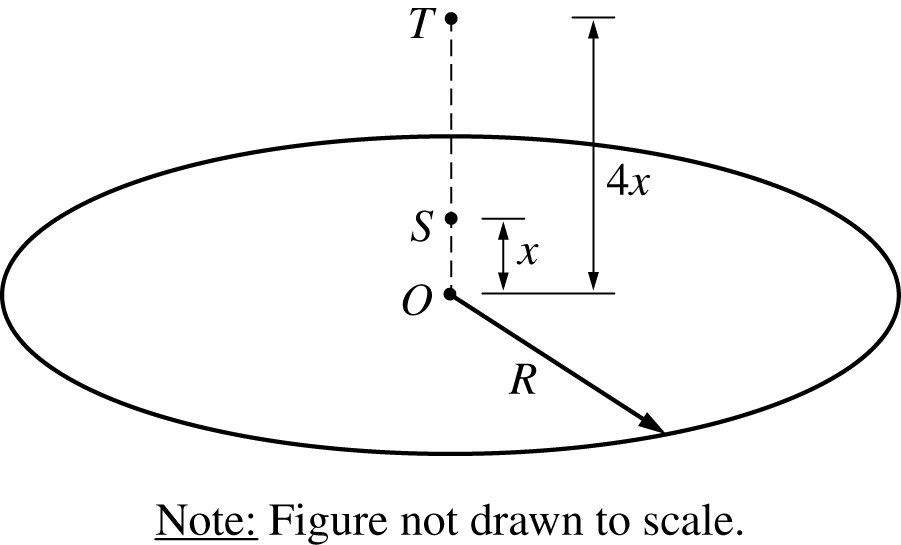
\includegraphics[scale=0.3]{images/img-005-005.png}
\end{figure}

The figure above shows a thin, circular nonconducting sheet of positive charge uniformly distributed over its area. The radius of the sheet is $R$. Point $O$ is at the center of the sheet. Point $S$ is a distance $x$ from the center of the sheet, and point $T$ is a distance $4 x$ from the center of the sheet.
Assume $R \gg x$.

% Multiple Choice Question 10
\begin{questions}\setcounter{question}{9}\question
If the magnitude of the electric field at point $T$ is $E_{T}$, which of the following best represents the magnitude of the electric field at point $S$ ?

\begin{oneparchoices}
\choice $E_{T} / 16$
\choice $E_{T} / 4$
\choice $E_{T}$
\choice $4 E_{T}$
\choice $16 E_{T}$
\end{oneparchoices}\end{questions}

% Multiple Choice Question 11
\begin{questions}\setcounter{question}{10}\question
A small sphere of mass $m$ and charge $-q$ is released from rest at point $T$. If the electric potentials at points $S$ and $T$ are $V_{S}$ and $V_{T}$, respectively, what is the speed of the sphere when it reaches point $S$ ? Ignore the effects of gravity.

\begin{choices}
\choice $\dfrac{2 q}{m}\left(V_{S}+V_{T}\right)$
\choice $\dfrac{4 q}{m}\left(V_{S}+V_{T}\right)$
\choice $\sqrt{\dfrac{q}{2 m}\left(V_{S}-V_{T}\right)}$
\choice $\sqrt{\dfrac{q}{2 m}\left(V_{S}+V_{T}\right)}$
\choice $\sqrt{\dfrac{2 q}{m}\left(V_{S}-V_{T}\right)}$
\end{choices}\end{questions}
